\documentclass[11pt]{article}

\usepackage[margin=1in]{geometry}
\usepackage{amsmath}
\usepackage{amssymb}
\usepackage{graphicx}
\usepackage{iftex}
\usepackage{tikz}
\usetikzlibrary{arrows.meta,positioning,shapes.geometric}

\ifPDFTeX
  \usepackage{newtxtext}
  \usepackage{newtxmath}
\else
  \usepackage{fontspec}
  \setmainfont{Times New Roman}
  \setsansfont{Times New Roman}
  \setmonofont{Times New Roman}
\fi

\setlength{\parindent}{0pt}
\setlength{\parskip}{0.5em}
\linespread{1.03}

\begin{document}

\begin{center}
{\LARGE Reroute Method Overview}\\[0.35em]
{\large Current waypoint-level multi-hazard reroute in the planning module}
\end{center}

\section*{Global Route Context}
\begin{minipage}[t]{0.59\textwidth}
\textbf{Initial route}

At the beginning of the scenario, the ego vehicle follows the stored global route from the start position to the final destination:
\[
\pi_{\mathrm{init}} = [w_0,w_1,\ldots,w_N]
\]
This initial route is already available in the planner stack and is tracked by the MPC controller.

\textbf{When reroute is triggered}

The behavior planner reads cooperative messages from \texttt{cp\_message.json}. A lane-closure message can trigger
\[
\text{decision}=\texttt{reroute}
\]
when the reported hazard lies on the current route and is ahead of the ego vehicle.

This reroute check is evaluated before the planner splits into \texttt{NORMAL} and \texttt{INTERSECTION}, so the same reroute decision can be taken in both modes.

\textbf{Important runtime detail}

The lane-closure messages are not deleted after the first check. When reroute executes, the runner reloads the full current set of \texttt{lane\_closure} messages, so all active hazards are considered together.
\end{minipage}
\hfill
\begin{minipage}[t]{0.36\textwidth}
\centering
\textbf{Pipeline}\\[0.4em]
\resizebox{0.98\textwidth}{!}{
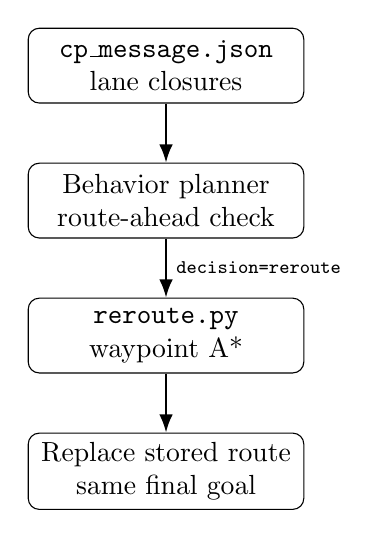
\begin{tikzpicture}[
  node distance=0.75cm,
  box/.style={
    draw,
    rounded corners,
    align=center,
    minimum width=3.5cm,
    minimum height=0.95cm
  },
  line/.style={-Latex,thick}
]
\node[box] (msg) {\texttt{cp\_message.json}\\lane closures};
\node[box,below=of msg] (bp) {Behavior planner\\route-ahead check};
\node[box,below=of bp] (rr) {\texttt{reroute.py}\\waypoint A*};
\node[box,below=of rr] (gp) {Replace stored route\\same final goal};

\draw[line] (msg) -- (bp);
\draw[line] (bp) -- node[right] {\scriptsize \texttt{decision=reroute}} (rr);
\draw[line] (rr) -- (gp);
\end{tikzpicture}
}

\vspace{0.7em}
\textbf{Message fields}
\begin{itemize}
\setlength\itemsep{0.25em}
\item \texttt{id}
\item \texttt{position = [x,y]}
\item \texttt{road\_id}
\item \texttt{lane\_id}
\item \texttt{carla\_lane\_id} if available
\end{itemize}
\end{minipage}

\clearpage
\section*{Hazard Resolution and Blocked Footprint}
\begin{minipage}[t]{0.59\textwidth}
\textbf{Per-hazard preprocessing}

For each \texttt{lane\_closure} message, the reroute method performs the following steps:
\begin{itemize}
\setlength\itemsep{0.3em}
\item Snap the reported \texttt{position} to the nearest CARLA driving waypoint.
\item Compare the message \texttt{road\_id} and \texttt{lane\_id} with the snapped CARLA waypoint.
\item If the message identifiers are incompatible with CARLA, normalize them locally inside reroute using the snapped waypoint.
\item Build a stable waypoint key for A*:
\[
k(w)=\bigl(\text{road id},\text{section id},\text{raw lane id},\mathrm{round}(s)\bigr)
\]
\item If the longitudinal coordinate \(s\) is unavailable, the implementation falls back to rounded \((x,y)\) values.
\end{itemize}

\textbf{Blocked footprint}

The current method does not block an entire road or lane. Instead, each hazard blocks a short footprint on its lane:
\[
B_i=\{w^{(i)}_{-2},w^{(i)}_{-1},w^{(i)}_0,w^{(i)}_{+1},w^{(i)}_{+2}\}
\]
where \(w^{(i)}_0\) is the snapped hazard waypoint, two waypoints are taken from \texttt{next(...)} and two from \texttt{previous(...)}.

For multiple hazards, the blocked set used by A* is the union
\[
B=\bigcup_{i=1}^{M} B_i
\]
so all active hazards are blocked simultaneously before search begins.
\end{minipage}
\hfill
\begin{minipage}[t]{0.36\textwidth}
\centering
\textbf{Five-waypoint block footprint}\\[0.4em]
\resizebox{0.98\textwidth}{!}{
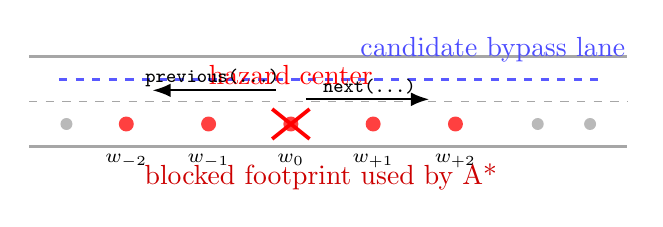
\begin{tikzpicture}[x=0.95cm,y=0.95cm]
  \draw[gray!70, line width=1.0pt] (0,1.25) -- (8,1.25);
  \draw[gray!70, dashed] (0,0.65) -- (8,0.65);
  \draw[gray!70, line width=1.0pt] (0,0.05) -- (8,0.05);

  \draw[blue!65,dashed,line width=1.0pt] (0.4,0.95) -- (7.6,0.95);
  \node[blue!70] at (6.2,1.35) {candidate bypass lane};

  \foreach \x/\lbl in {
    1.3/$w_{-2}$,
    2.4/$w_{-1}$,
    3.5/$w_0$,
    4.6/$w_{+1}$,
    5.7/$w_{+2}$
  } {
    \fill[red!75] (\x,0.35) circle (0.10);
    \node[below] at (\x,0.08) {\scriptsize \lbl};
  }
  \foreach \x in {0.5,6.8,7.5} {
    \fill[gray!55] (\x,0.35) circle (0.08);
  }

  \draw[red, line width=1.35pt] (3.25,0.15) -- (3.75,0.55);
  \draw[red, line width=1.35pt] (3.25,0.55) -- (3.75,0.15);
  \node[red] at (3.5,1.0) {hazard center};

  \draw[-Latex,thick] (3.7,0.68) -- (5.35,0.68);
  \node at (4.55,0.85) {\scriptsize \texttt{next(...)}};

  \draw[-Latex,thick] (3.3,0.80) -- (1.65,0.80);
  \node at (2.45,0.97) {\scriptsize \texttt{previous(...)}};

  \node[red!80!black] at (3.9,-0.35) {blocked footprint used by A*};
\end{tikzpicture}
}
\end{minipage}

\clearpage
\section*{Waypoint-Level A* Search}
\begin{minipage}[t]{0.59\textwidth}
\textbf{Search space}

The reroute search is performed directly on CARLA driving waypoints. The reroute function does not call the CARLA global planner to search for the new path.

\textbf{Start and goal}
\begin{itemize}
\setlength\itemsep{0.3em}
\item Start node: the ego vehicle's current driving waypoint.
\item Goal node: the scenario final destination snapped to an unblocked driving waypoint.
\item If the ego start lane is blocked, the method can retry from an adjacent unblocked ego lane.
\end{itemize}

\textbf{Neighbors and costs}

From a waypoint \(w\), the A* expansion uses:
\[
\mathcal{N}(w)=\{w'\in w.\texttt{next}(d)\}\cup\{w_L,w_R\}
\]
where \(w_L\) and \(w_R\) are same-direction adjacent lane waypoints.

\[
c(w,w')=
\begin{cases}
d, & \text{forward step}\\[0.3em]
2.5d, & \text{lane-change step}
\end{cases}
\]

\textbf{A* objective}
\[
f(w)=g(w)+h(w), \qquad
h(w)=\|p(w)-p(w_{\mathrm{goal}})\|_2
\]
Any candidate waypoint whose key belongs to the blocked set \(B\) is skipped.
\end{minipage}
\hfill
\begin{minipage}[t]{0.36\textwidth}
\centering
\textbf{A* detour around blocked waypoints}\\[0.4em]
\resizebox{0.98\textwidth}{!}{
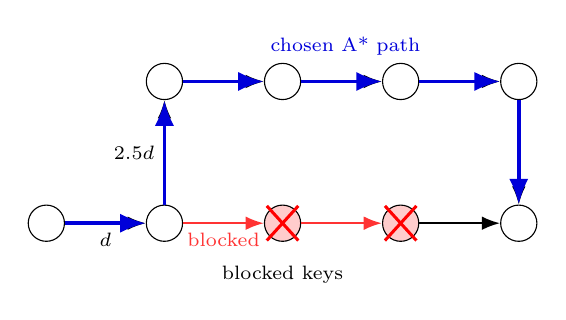
\begin{tikzpicture}[x=1.0cm,y=1.0cm]
  \tikzstyle{vtx}=[circle,draw,minimum size=0.46cm,inner sep=0pt]

  \node[vtx] (a) at (0,0) {};
  \node[vtx] (b) at (1.5,0) {};
  \node[vtx,fill=red!20] (c) at (3.0,0) {};
  \node[vtx,fill=red!20] (d) at (4.5,0) {};
  \node[vtx] (e) at (6.0,0) {};

  \node[vtx] (u1) at (1.5,1.8) {};
  \node[vtx] (u2) at (3.0,1.8) {};
  \node[vtx] (u3) at (4.5,1.8) {};
  \node[vtx] (u4) at (6.0,1.8) {};

  \draw[-Latex,thick] (a) -- node[below] {\scriptsize $d$} (b);
  \draw[-Latex,thick,red!80] (b) -- node[below] {\scriptsize blocked} (c);
  \draw[-Latex,thick,red!80] (c) -- (d);
  \draw[-Latex,thick] (d) -- (e);

  \draw[-Latex,thick] (u1) -- (u2);
  \draw[-Latex,thick] (u2) -- (u3);
  \draw[-Latex,thick] (u3) -- (u4);

  \draw[-Latex,thick,dashed] (b) -- node[left] {\scriptsize $2.5d$} (u1);
  \draw[-Latex,thick,dashed] (u4) -- (e);

  \draw[blue!85!black,line width=1.4pt,-Latex] (a) -- (b);
  \draw[blue!85!black,line width=1.4pt,-Latex] (b) -- (u1);
  \draw[blue!85!black,line width=1.4pt,-Latex] (u1) -- (u2);
  \draw[blue!85!black,line width=1.4pt,-Latex] (u2) -- (u3);
  \draw[blue!85!black,line width=1.4pt,-Latex] (u3) -- (u4);
  \draw[blue!85!black,line width=1.4pt,-Latex] (u4) -- (e);

  \draw[red, line width=1.1pt] (2.8,-0.22) -- (3.2,0.22);
  \draw[red, line width=1.1pt] (2.8,0.22) -- (3.2,-0.22);
  \draw[red, line width=1.1pt] (4.3,-0.22) -- (4.7,0.22);
  \draw[red, line width=1.1pt] (4.3,0.22) -- (4.7,-0.22);

  \node at (3.0,-0.65) {\scriptsize blocked keys};
  \node[blue!85!black] at (3.8,2.25) {\scriptsize chosen A* path};
\end{tikzpicture}
}
\end{minipage}

\clearpage
\section*{How the New Route Is Found}
\textbf{Step 1}

Read the current \texttt{lane\_closure} messages from \texttt{cp\_message.json} and keep the hazards that lie on the active route ahead of the ego vehicle.

\textbf{Step 2}

For each hazard, snap the reported position to the nearest CARLA driving waypoint. If the message \texttt{road\_id} or \texttt{lane\_id} does not match CARLA, normalize it locally using the snapped waypoint.

\textbf{Step 3}

Expand each snapped hazard to a blocked waypoint footprint:
\[
B_i=\{w^{(i)}_{-2},w^{(i)}_{-1},w^{(i)}_0,w^{(i)}_{+1},w^{(i)}_{+2}\}
\]
and merge all hazards into one blocked set
\[
B=\bigcup_{i=1}^{M} B_i
\]

\textbf{Step 4}

Run waypoint-level A* from the ego waypoint to an unblocked goal waypoint:
\[
\pi_{\mathrm{new}}
=
\operatorname{A^*}_{\,B\ \mathrm{blocked}}
\left(w_{\mathrm{ego}},w_{\mathrm{goal}}\right)
\]
Forward neighbors come from \texttt{next(d)} and same-direction lane-change neighbors come from left/right adjacent lanes. If needed, retry from an adjacent unblocked ego lane.

\textbf{Step 5}

If a valid route is found and it avoids all blocked waypoint keys, convert the waypoint path to route points and replace the stored global route.

\end{document}
